\section{Primera revisión de los datos}\label{sec:exploracion}
Antes de construir un modelo revisamos los datos con cálculos sencillos. Lo que sigue son observaciones
preliminares. Antes de usarlas para decidir algo, alguien que no las haya calculado debe reproducirlas desde los
archivos originales (Tabla~\ref{tab:verificar}).

\subsection{Dos formas de medir el rendimiento}
La Fig.~\ref{fig:regimenes} muestra el rendimiento de cada parcela por municipio. En cuatro municipios los valores
tienen dos decimales, como 4.47 o 4.52, y rondan 4.5~t/ha. En los otros cinco están redondeados a escalones de media
tonelada, como 2.5, 3.0 o 3.5, y rondan 3~t/ha. Llamamos \emph{régimen A} al primer grupo y \emph{régimen B} al
segundo (Tabla~\ref{tab:regimenes}).

\begin{figure*}[!t]
\centering
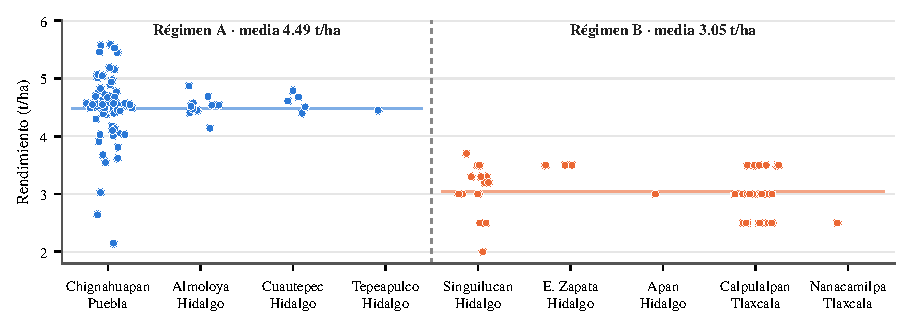
\includegraphics[width=\textwidth]{fig_regimenes}
\caption{Rendimiento de las 138 parcelas de entrenamiento por municipio. El color indica el régimen. En el régimen B
los valores se apilan en escalones de media tonelada.}\label{fig:regimenes}
\end{figure*}

\begin{table}[!t]
\caption{Rendimiento de entrenamiento por régimen}\label{tab:regimenes}
\centering\footnotesize
\begin{tabularx}{\columnwidth}{@{}lXrr@{}}
\toprule
Rég. & Municipios & Parcelas & Media (t/ha) \\
\midrule
A & Chignahuapan, Almoloya, Cuautepec de Hinojosa, Tepeapulco & 87 & 4.49 \\
B & Singuilucan, Emiliano Zapata, Apan, Calpulalpan, Nanacamilpa & 51 & 3.05 \\
\bottomrule
\end{tabularx}
\end{table}

\textbf{La separación no coincide con el estado.} El régimen se define por cómo está escrito el número, con decimales
o redondeado, y no por su valor. Hidalgo tiene municipios de los dos tipos. Almoloya, Cuautepec de Hinojosa y
Tepeapulco se parecen a Puebla, y Singuilucan, Emiliano Zapata y Apan se parecen a Tlaxcala. Agrupar por estado
mezcla dos poblaciones dentro de Hidalgo. El municipio también se conoce para las 59 parcelas de predicción, así que
el régimen se puede usar como variable.

\textbf{La causa todavía no es clara.} La diferencia puede ser real o puede deberse a la forma de medir. La
estadística oficial de 2025 va en sentido contrario a las etiquetas (Tabla~\ref{tab:siap}), lo que apunta a la forma
de medir. Por otro lado, las curvas de verdor sugieren que en el régimen B el ciclo es más corto, lo que podría
reflejar otra variedad o fecha de siembra. Para predecir, la causa importa poco, porque las 59 parcelas se califican
con etiquetas medidas igual que las de su municipio. Para interpretar los resultados sí importa, y conviene
preguntarlo a los organizadores.

\begin{table}[!t]
\caption{Media del reto y rendimiento municipal oficial de 2025, cebada de temporal~\cite{siap2026}}\label{tab:siap}
\centering\footnotesize
\begin{tabular}{@{}llrr@{}}
\toprule
Municipio & Rég. & Reto & SIAP 2025 \\
\midrule
Chignahuapan & A & 4.48 & 3.22 \\
Almoloya & A & 4.52 & 1.91 \\
Cuautepec de Hinojosa & A & 4.60 & 2.35 \\
Calpulalpan & B & 3.00 & 4.00 \\
Singuilucan & B & 3.08 & 1.88 \\
\bottomrule
\end{tabular}
\end{table}

\subsection{Valores extremos en parcelas pequeñas}
De los cinco rendimientos más altos, todos de 5.4~t/ha o más, cuatro son de parcelas de menos de 1.5 hectáreas
(Fig.~\ref{fig:area}). Con mediciones de campo se ha documentado que los productores sobreestiman el rendimiento
sobre todo en parcelas pequeñas~\cite{gourlay2019}. Si aquí pasa lo mismo, parte de esos valores es ruido de
etiqueta y no algo que el satélite pueda explicar.

\begin{figure}[!t]
\centering
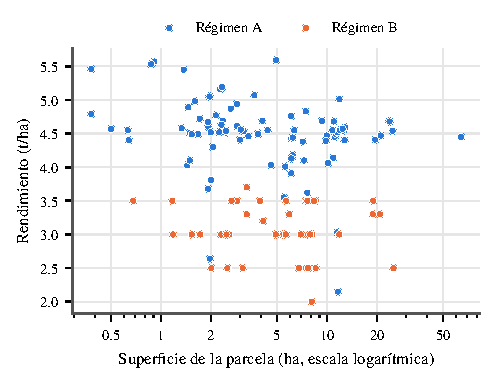
\includegraphics[width=\columnwidth]{fig_area}
\caption{Rendimiento frente al tamaño de la parcela, en escala logarítmica. Cuatro de los cinco rendimientos de
5.4~t/ha o más corresponden a parcelas de menos de 1.5 hectáreas.}\label{fig:area}
\end{figure}

\subsection{Error por redondeo}
Redondear a la media tonelada más cercana agrega por sí solo un error típico de unos 0.14~t/ha, si el valor real
puede caer en cualquier punto del escalón. En el régimen B ningún modelo podría bajar de ese error, aunque fuera
perfecto.

\subsection{La lluvia de 2025}
A nivel nacional, 2025 fue el año más lluvioso desde 1941. En la zona de las parcelas el total de junio a octubre fue
parecido al de 2024, y lo que cambió fue el momento de la lluvia (Fig.~\ref{fig:lluvia} y Tabla~\ref{tab:lluvia}).
\begin{enumerate}
  \item \textbf{Mayo y junio fueron muy lluviosos}, con el doble de lluvia que cualquiera de los tres años
        anteriores. Eso favorece sembrar a tiempo, pero puede encharcar las parcelas recién sembradas.
  \item \textbf{Julio y agosto fueron normales}, sin exceso durante el llenado de grano.
  \item \textbf{Septiembre y octubre volvieron a ser lluviosos}, en la madurez y la cosecha. En esa etapa la lluvia
        puede tumbar el cultivo, lo que se conoce como \emph{acame}, o retrasar la cosecha.
  \item \textbf{La temperatura máxima fue más fresca} que en 2023 y 2024, lo que suele favorecer el llenado del
        grano.
\end{enumerate}
Esto sugiere que los efectos del exceso de agua fueron de parcela, en zonas bajas o en parcelas cosechadas tarde, y
no de zona. El clima mensual de 5 kilómetros difícilmente los detecta.

\begin{figure}[!t]
\centering
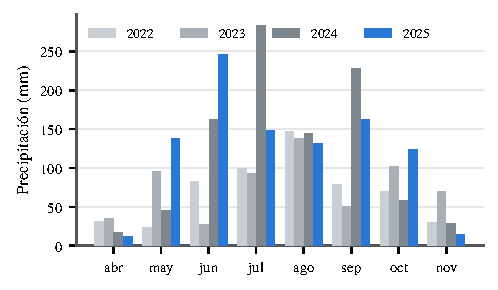
\includegraphics[width=\columnwidth]{fig_lluvia}
\caption{Precipitación mensual promedio sobre las 197 parcelas, de abril a noviembre~\cite{funk2015}.}\label{fig:lluvia}
\end{figure}

\begin{table}[!t]
\caption{Lluvia por etapa y temperatura máxima, promedio sobre las parcelas}\label{tab:lluvia}
\centering\footnotesize
\begin{tabular}{@{}lrrrr@{}}
\toprule
 & 2022 & 2023 & 2024 & 2025 \\
\midrule
Mayo y junio (mm) & 106 & 122 & 207 & \textbf{384} \\
Julio y agosto (mm) & 246 & 231 & 427 & 281 \\
Septiembre y octubre (mm) & 148 & 154 & 287 & \textbf{286} \\
Tmax de mayo a sep. (°C) & 23.7 & 24.7 & 25.0 & 23.6 \\
\bottomrule
\end{tabular}
\end{table}

\subsection{Verificación}
La Tabla~\ref{tab:verificar} indica cómo comprobar cada observación. Si los números de quien las reproduce coinciden,
la observación pasa a ser un hecho.

\begin{table}[!t]
\caption{Observaciones preliminares y cómo comprobarlas}\label{tab:verificar}
\centering\footnotesize
\begin{tabularx}{\columnwidth}{@{}>{\raggedright\arraybackslash}p{3.3cm}X@{}}
\toprule
Observación & Cómo comprobarla \\
\midrule
Dos regímenes de medición por municipio & Contar por municipio los rendimientos con dos decimales y calcular la
  media de cada grupo \\
El régimen separa mejor que el estado & Comparar la varianza explicada por cada agrupación \\
Valores extremos en parcelas pequeñas & Graficar rendimiento contra área y revisar las cinco parcelas más altas \\
Lluvia de 2025 concentrada en siembra y cosecha & Extraer CHIRPS por parcela y sumar por bimestre y año \\
Más observaciones limpias en 2025 & Contar por año las fechas con nubosidad baja entre mayo y octubre \\
Planet cubre todo 2025 & Convertir las fechas con formato día, mes y año y revisar el rango \\
Ciclo más corto en el régimen B & Estimar inicio y fin del verdor por parcela y comparar entre regímenes \\
\bottomrule
\end{tabularx}
\end{table}
